\documentclass{article}[12pt]

\usepackage{graphicx}
\usepackage{gensymb}

\begin{document}
	
\section{10/04 Observation Date}
	
\begin{table}[h]
	\begin{center}
	\begin{tabular}{|c | c | c | c | c |}
		\hline
		Nebula Name & RA & Dec & Magnitude & Alt. at 10pm \\
		\hline
		\hline
		M 27 & $299.9\degree$ & $+22.72\degree$ & 7.3 & $59.5\degree$\\
		\hline
	\end{tabular}
	\end{center}
\end{table}

\begin{figure}[h]
	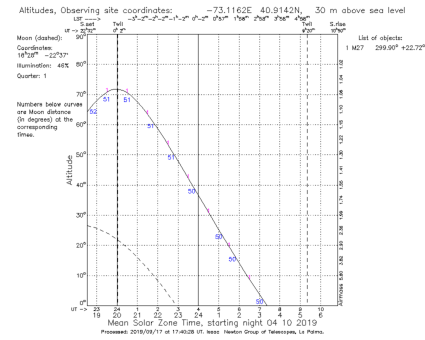
\includegraphics[width=\linewidth]{M27_10_04.pdf}
\end{figure}

\newpage

\section{10/18 Observation Date}

\begin{table}[h]
	\begin{center}
		\begin{tabular}{|c | c | c | c | c |}
			\hline
			Nebula Name & RA & Dec & Magnitude & Alt. at 10pm \\
			\hline
			\hline
			NGC 6826 & $296.2\degree$ & $+50.52\degree$ & 8.8 & $56.5\degree$\\
			\hline
		\end{tabular}
	\end{center}
\end{table}

\begin{figure}[h]
	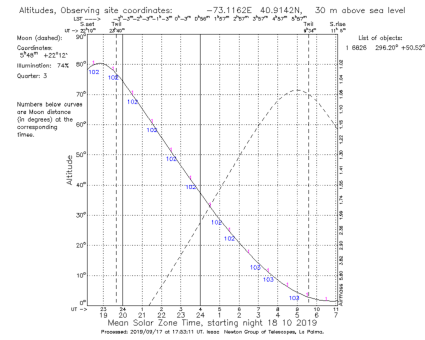
\includegraphics[width=\linewidth]{NGC6826_10_18.pdf}
\end{figure}

\newpage

\section{10/22 Observation Date}

\begin{table}[h]
	\begin{center}
		\begin{tabular}{|c | c | c | c | c |}
			\hline
			Nebula Name & RA & Dec & Magnitude & Alt. at 10pm \\
			\hline
			\hline
			NGC 7662 & $351.5\degree$ & $+42.55\degree$ & 8.6 & $86.1\degree$\\
			\hline
		\end{tabular}
	\end{center}
\end{table}

\begin{figure}[h]
	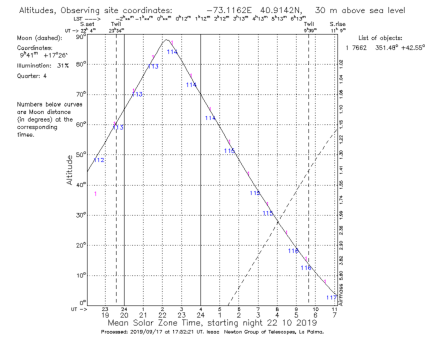
\includegraphics[width=\linewidth]{NGC7662_10_22.pdf}
\end{figure}


\end{document}